\documentclass[11pt,a4paper]{article}
\usepackage[T1]{fontenc}
\usepackage[margin=2.3cm]{geometry}
\usepackage{amsmath,amssymb}
\usepackage{graphicx}
\usepackage[dvipsnames]{xcolor}
\usepackage{enumitem}
\usepackage[colorlinks=true,linkcolor=blue,urlcolor=blue]{hyperref}
\setlength{\parskip}{0.6em}
\setlength{\parindent}{0pt}
\begin{document}

\begin{center}{\LARGE\bfseries openlinkage}\\[0.4em]{\large Design a four-bar walking machine, Strandbeest style, in three sessions.}\\[0.2em]\small PAN IIT OSS explainer \textbullet{} diploma / undergraduate to advanced undergraduate (levels 5-6)\end{center}

\section*{Why this exists}
A walking machine can be made of nothing but rigid bars and pins. This explainer shows the mathematics behind it: two circles that place a pin, a rule that says whether a crank can turn, and a measurement of how straight a foot moves, so that you can design a leg yourself.

\section*{The end goal}
Design a four-bar walking machine (Strandbeest style). The end goal is a four-bar walking machine in the style of Theo Jansen's Strandbeest: legs made of linkages, one crank per leg, a foot that moves along a nearly straight line while it is on the ground. The same mathematics drives wipers, pumps, robot grippers and suspensions.

\section*{How the three sessions build up}
\begin{enumerate}[nosep]
\item \textbf{Session 1: Four bars, four pins, one motion} (Level 1, conceptual interactive model, 60 min).
\item \textbf{Session 2: The four-bar linkage as equations} (Level 2, mathematical engineering model, 75 min).
\item \textbf{Session 3: A walking leg: simulate, validate and tune} (Level 3, simulation and validation, 90 min).
\end{enumerate}

\section{Session 1: Four bars, four pins, one motion}

\subsection*{A. Real-world problem}
A windscreen wiper, a walking toy and a bicycle suspension all move by rigid bars joined at pins. Nobody pushes every bar: one motor turns one bar (the crank) and all the others follow in a fixed way. Even stranger, a point on the middle bar (the coupler) draws a curve, and that curve can be shaped to be almost straight, which is how some walking machines move their feet. How can a few stiff bars, joined at four pins, turn one steady rotation into a rocking motion and a looping path?

\subsection*{B. Concept and theory}
The frame (ground bar) holds two fixed pins O2 at (0, 0) and O4 at (a, 0). The crank (length b) turns about O2, so its free end A is at b(cos t, sin t). The coupler (length c) joins A to a pin B, and the rocker (length d) joins B to O4. So B is at distance c from A and at distance d from O4: it is where two circles cross. Two circles usually cross in two points, so there are two ways to assemble the linkage; we take the one to the left of the line from A to O4. Once the crank angle t is chosen, A, B and the rocker angle are all fixed: the linkage has one freedom. A plane bar has 3 freedoms (x, y, angle); a pin removes 2, and the ground bar is fixed, so n bars and j pins leave M = 3(n - 1) - 2j freedoms. For the four-bar, M = 3*3 - 2*4 = 1. At the extreme positions of the rocker, the crank and the coupler lie on one line, so B is at distance c + b or c - b from O2; the law of cosines then gives the rocker's swing.

\begin{itemize}[nosep]
\item a: ground bar: distance O2 to O4 (a, b, c, d are lengths in any one unit) (length units)
\item b: crank length (O2 to A) (length units)
\item c: coupler length (A to B) (length units)
\item d: rocker length (O4 to B) (length units)
\item t: crank angle, from the +x axis (degrees)
\item k: coupler point P = A + k (B - A), k = 0.5 is the middle (no unit)
\item n, j, M: number of bars, number of pins, number of freedoms (no unit)
\end{itemize}

\begin{equation*}
\mathbf A=b(\cos t,\ \sin t),\qquad \lVert\mathbf B-\mathbf A\rVert=c,\qquad \lVert\mathbf B-\mathbf O_4\rVert=d
\end{equation*}

\begin{equation*}
M=3(n-1)-2j\qquad(\text{four-bar: }3\cdot 3-2\cdot 4=1)
\end{equation*}

\begin{equation*}
\cos\psi=\frac{a^2+d^2-r^2}{2ad},\qquad r=c+b\ \text{or}\ c-b\ \text{(the two extreme positions)}
\end{equation*}

\begin{equation*}
\text{swing}=\left|\psi_{c+b}-\psi_{c-b}\right|
\end{equation*}

\begin{center}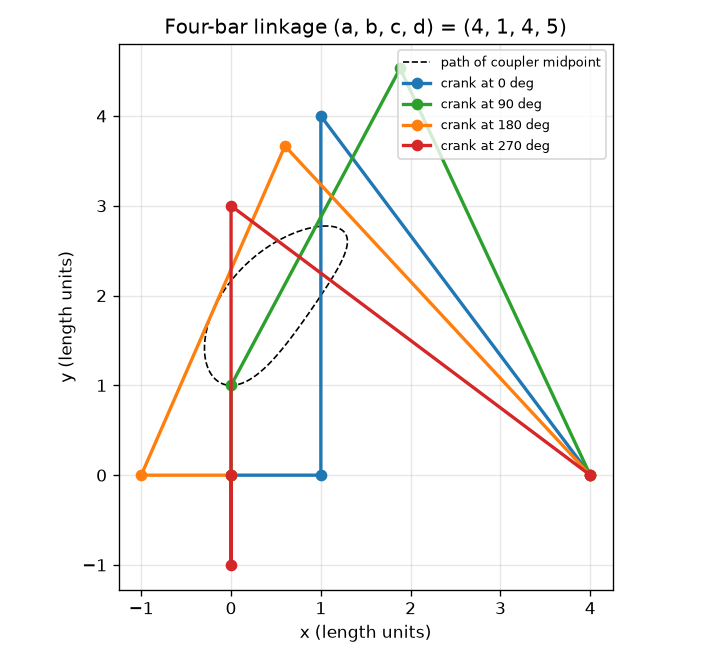
\includegraphics[width=0.85\linewidth]{figures/s01_linkage_poses.png}\\\small The linkage (4, 1, 4, 5) at four crank angles, with the path of the coupler midpoint.\end{center}

\subsection*{E. Worked example}
For (a, b, c, d) = (4, 1, 4, 5) find the pin B and the rocker angle when the crank lies along the ground bar (t = 0). Then find the rocker's total swing.
\begin{enumerate}[nosep]
\item At t = 0 the crank tip is A = (1, 0). The rocker pivot is O4 = (4, 0), so A is 3 units from O4.
\item B is 4 from A and 5 from O4. A triangle with sides 3, 4, 5 has a right angle between the sides 3 and 4, so B is straight above A: B = (1, 4).
\item The rocker points from O4 = (4, 0) to B = (1, 4), the vector (-3, 4). Its angle from the +x axis is atan2(4, -3) = 126.87 degrees.
\item Extremes: \textbar{}O2 B\textbar{} = c + b = 5 gives cos(psi) = (16 + 25 - 25)/40 = 0.4, psi = 66.42 degrees; \textbar{}O2 B\textbar{} = c - b = 3 gives cos(psi) = (16 + 25 - 9)/40 = 0.8, psi = 36.87 degrees.
\item Swing = 66.42 - 36.87 = 29.55 degrees. A sampled check of the rocker angle over a full turn gives the same swing.
\end{enumerate}
\textbf{Answer.} B = (1, 4), rocker angle 126.87 degrees at t = 0, and the rocker swings through 29.55 degrees (between 113.58 and 143.13 degrees).

\subsection*{F. Questions}
\begin{enumerate}[nosep]
\item \textbf{Conceptual.} Why does turning only the crank decide the position of the coupler and the rocker as well? What would have to be different for the linkage to need two motors?
\item \textbf{Numerical.} For (a, b, c, d) = (4, 1, 4, 5) find the pin B and the rocker angle when the crank angle is 180 degrees.
\item \textbf{Graph and simulation interpretation.} In the graph of rocker angle against crank angle, at which crank angles is the rocker at its two extreme positions, and how large is the swing?
\item \textbf{Design and optimisation challenge.} Design: with a = 4, c = 4 and d = 5 the rocker must swing through at least 40 degrees. Choose a crank length from 1.0, 1.5 and 2.0 and justify your choice.
\end{enumerate}

\section{Session 2: The four-bar linkage as equations}

\subsection*{A. Real-world problem}
A workshop needs a crank that turns round and round to rock an output arm through exactly 40 degrees. Which bar lengths do we choose? Three questions decide it. Can the crank turn a full circle at all, or will it jam? Where is every pin for a given crank angle? And when the coupler pushes the rocker, does the push turn the rocker or just squeeze the pin? A linkage that swings correctly on paper can still lock in practice.

\subsection*{B. Concept and theory}
Name the bars ground a, crank b, coupler c, rocker d. Let s be the shortest, l the longest and p, q the other two. Grashof's rule: if s + l \textless{}= p + q, the shortest bar can make a full turn relative to its neighbours. Where the shortest bar sits decides the kind of motion: crank b gives a crank-rocker, ground a a double-crank, coupler c a double-rocker. If s + l \textgreater{} p + q no bar turns fully (triple-rocker), and equality is the change-point case. The position problem is solved by the circle crossing of Session 1, or by the loop-closure equation: walking round the loop O2, A, B, O4 returns to the start, which gives two equations for the two unknown angles of the coupler and the rocker (Newton's method solves them from a guess). The transmission angle mu is the angle between coupler and rocker at B: with D the distance from A to O4, cos(mu) = (c\textasciicircum{}2 + d\textasciicircum{}2 - D\textasciicircum{}2)/(2cd). At mu = 90 degrees all the push turns the rocker; near 0 or 180 degrees most of it squeezes the pin. A common design guideline keeps mu between about 40 and 140 degrees; it is a rule of thumb, not a law.

\begin{itemize}[nosep]
\item a, b, c, d: ground, crank, coupler, rocker lengths (length units)
\item s, l, p, q: shortest, longest and the two other bar lengths (length units)
\item t2, t3, t4: angles of the crank, coupler and rocker from the +x axis (radians)
\item mu: transmission angle between coupler and rocker at B (degrees)
\item D: distance from the crank tip A to the rocker pivot O4 (length units)
\item psi: rocker angle measured from the ground line at O4 (degrees)
\end{itemize}

\begin{equation*}
s+l\le p+q\ \Rightarrow\ \text{the shortest bar can turn fully}
\end{equation*}

\begin{equation*}
b\,e(t_2)+c\,e(t_3)-d\,e(t_4)-(a,0)=(0,0),\qquad e(t)=(\cos t,\sin t)
\end{equation*}

\begin{equation*}
\cos\mu=\frac{c^2+d^2-D^2}{2cd}
\end{equation*}

\begin{equation*}
\text{swing}=\left|\arccos\frac{a^2+d^2-(c+b)^2}{2ad}-\arccos\frac{a^2+d^2-(c-b)^2}{2ad}\right|
\end{equation*}

\begin{center}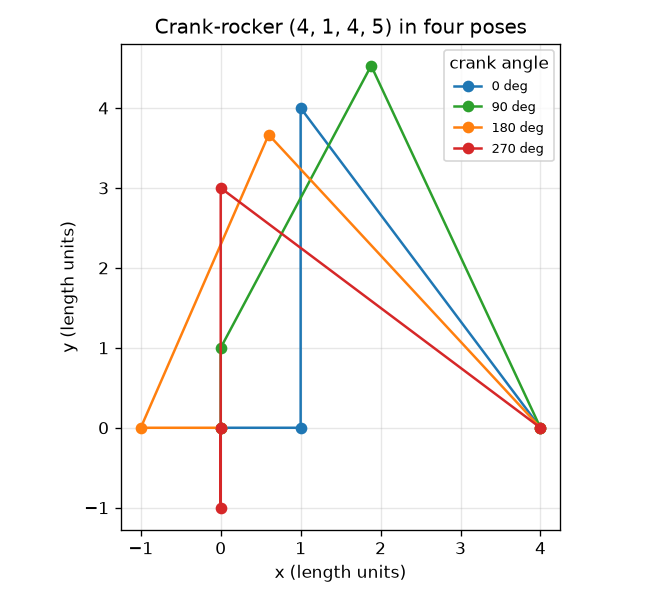
\includegraphics[width=0.85\linewidth]{figures/s02_crank_rocker_poses.png}\\\small The crank-rocker (4, 1, 4, 5) in four crank positions.\end{center}

\subsection*{E. Worked example}
For (a, b, c, d) = (4, 1, 4, 5) and a crank angle of 90 degrees find B, the transmission angle, and check Grashof's rule.
\begin{enumerate}[nosep]
\item Grashof: s = 1, l = 5, p + q = 4 + 4 = 8, and s + l = 6 \textless{}= 8. The shortest bar is the crank, so this is a crank-rocker.
\item At 90 degrees A = (0, 1) and O4 = (4, 0), so D\textasciicircum{}2 = 16 + 1 = 17 and D = 4.1231.
\item x = (c\textasciicircum{}2 - d\textasciicircum{}2 + D\textasciicircum{}2)/(2D) = (16 - 25 + 17)/8.2462 = 0.9701 and h = sqrt(16 - 0.9412) = 3.8806. The unit vector from A to O4 is (0.9701, -0.2425) and its left normal is (0.2425, 0.9701).
\item B = A + x e + h n = (0.9412 + 0.9412, 1 - 0.2353 + 3.7647) = (1.882, 4.529).
\item Transmission angle: cos(mu) = (c\textasciicircum{}2 + d\textasciicircum{}2 - D\textasciicircum{}2)/(2cd) = (16 + 25 - 17)/40 = 0.6, so mu = 53.13 degrees, inside the 40 to 140 degree guideline.
\end{enumerate}
\textbf{Answer.} B = (1.882, 4.529); the linkage is a crank-rocker; mu = 53.13 degrees at this crank angle.

\subsection*{F. Questions}
\begin{enumerate}[nosep]
\item \textbf{Conceptual.} Why does a linkage that satisfies Grashof's rule with the shortest bar as the coupler not let the crank turn a full circle?
\item \textbf{Numerical.} Classify the linkage (a, b, c, d) = (2, 5, 4, 6) with Grashof's rule. Which bar can turn fully?
\item \textbf{Graph and simulation interpretation.} In the transmission-angle graph for d = 5 (crank 1.346) the lowest point is 31.91 degrees. At which crank angle does it occur, and does the linkage meet the 40 to 140 degree guideline?
\item \textbf{Design and optimisation challenge.} Design: with a = 4 and c = 4 you may choose the rocker length d = 5 or d = 3.5. In each case find the crank length for a 40 degree swing, and choose one. Justify your choice.
\end{enumerate}

\section{Session 3: A walking leg: simulate, validate and tune}

\subsection*{A. Real-world problem}
Theo Jansen's beach walkers and many walking toys move on legs that are only bars and pins. The foot is a point on the coupler. For a smooth walk the foot must move along an almost straight line while it is on the ground (the stance), so the body glides forward without bobbing. Then it must lift off and swing back WITHOUT digging into the ground. How straight can four bars make the stance? Why are the famous straight-line linkages not good legs? How far does the foot step and lift, and what happens when the bars are chosen badly and the crank locks?

\subsection*{B. Concept and theory}
Our leg is a four-bar with ground a, crank b = 1, coupler c = 3.5 and rocker d = 2.25, with the foot P on the extension of the coupler beyond B: P = A + k (B - A). Simulating means solving the position problem for many crank angles, then checking it (Validation 1): the loop-closure error must be below 1e-12 and the bar lengths must stay constant. Velocity is checked two ways (Validation 2). Finite differences move the crank a tiny step either side and divide. The analytic way differentiates the loop equation: for a crank speed w2 the coupler and rocker speeds w3, w4 solve a 2 by 2 linear system (the Jacobian), and the foot velocity follows. A third view uses the instant centre I24, where the coupler line meets the ground line: w4/w2 = x\_I/(x\_I - a). For an ideal linkage no power is lost, so torque\_in * w\_in = torque\_out * w\_out and the mechanical advantage is MA = w2/w4; statics (a two-force coupler) gives the same ratio from distances alone. A stance is a run of consecutive crank angles (180 degrees here, a duty factor of 0.5). Its deviation is the largest perpendicular distance of the foot from the best-fit straight line through the stance points; stride is the distance between the first and last stance point. In the rest of the cycle (the swing) the height above the stance line, positive towards the body, gives two numbers: lift (the highest point) and dig (how far the foot goes below the line, which would be inside the ground). Grashof's rule must hold for the crank to turn fully; if it fails, the crank locks at a dead centre where the coupler and rocker lie on one line (mu = 0 or 180 degrees).

\begin{itemize}[nosep]
\item a, b, c, d: ground, crank, coupler, rocker (b = 1 sets the length unit, 'crank length') (crank lengths)
\item k: foot position on the coupler: P = A + k (B - A) (no unit)
\item w2, w3, w4: angular speeds of crank, coupler, rocker (rad/s)
\item I24: instant centre: coupler line meets ground line at x\_I (crank lengths)
\item MA: mechanical advantage tau\_out / tau\_in = w2 / w4 (no unit)
\item deviation, stride: straightness of the stance and step length (crank lengths)
\item lift, dig: highest point of the swing above the stance line, and deepest point below it (crank lengths)
\item duty factor: stance fraction of the cycle (stance span / 360 degrees) (no unit)
\end{itemize}

\begin{equation*}
\mathbf P=\mathbf A+k(\mathbf B-\mathbf A),\qquad b\,e(t_2)+c\,e(t_3)=(a,0)+d\,e(t_4)
\end{equation*}

\begin{equation*}
\begin{pmatrix}-c\sin t_3 & d\sin t_4\\ c\cos t_3 & -d\cos t_4\end{pmatrix}\begin{pmatrix}\omega_3\\ \omega_4\end{pmatrix}=b\,\omega_2\begin{pmatrix}\sin t_2\\ -\cos t_2\end{pmatrix}
\end{equation*}

\begin{equation*}
\frac{\omega_4}{\omega_2}=\frac{x_I}{x_I-a},\qquad \tau_{\rm in}\omega_2=\tau_{\rm out}\omega_4\ \Rightarrow\ \mathrm{MA}=\frac{\omega_2}{\omega_4}
\end{equation*}

\begin{equation*}
\delta=\max_i\left|\mathbf n\cdot(\mathbf P_i-\bar{\mathbf P})\right|,\qquad \text{stride}=\lVert\mathbf P_{\rm last}-\mathbf P_{\rm first}\rVert
\end{equation*}

\begin{center}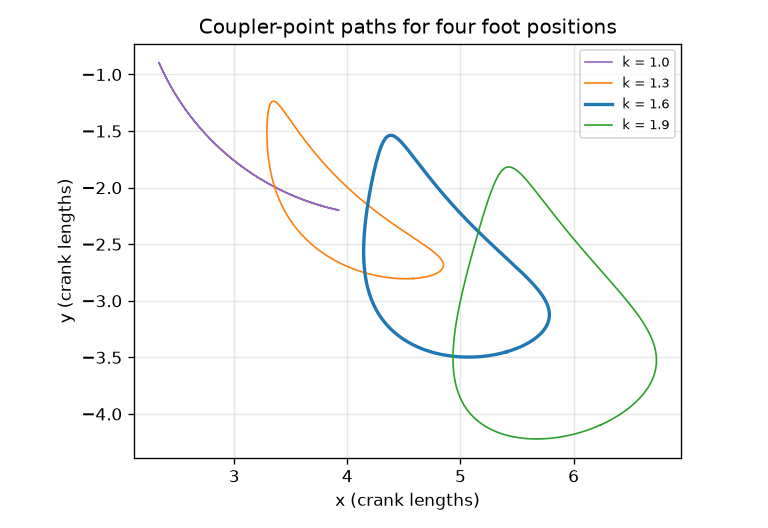
\includegraphics[width=0.85\linewidth]{figures/s03_coupler_paths.png}\\\small Coupler-point paths of the leg for four foot positions k.\end{center}

\subsection*{E. Worked example}
For the leg (a, b, c, d) = (4.4, 1, 3.5, 2.25) with k = 1.6, find B and the foot at crank angle 0, then the rocker speed ratio by the instant centre and the mechanical advantage.
\begin{enumerate}[nosep]
\item Crank angle 0: A = (1, 0), O4 = (4.4, 0), so D = 3.4. x = (c\textasciicircum{}2 - d\textasciicircum{}2 + D\textasciicircum{}2)/(2D) = (12.25 - 5.0625 + 11.56)/6.8 = 2.757 and h = sqrt(12.25 - 2.757\textasciicircum{}2) = 2.156.
\item The foot hangs below the frame (the -1 assembly): B = (1 + 2.757, -2.156) = (3.757, -2.156). The foot is P = A + 1.6 (B - A) = (1 + 4.411, -3.450) = (5.411, -3.450).
\item The coupler line passes through A, which lies on the ground line y = 0, so the instant centre is I24 = A = (1, 0), x\_I = 1.
\item w4/w2 = x\_I/(x\_I - a) = 1/(1 - 4.4) = -5/17 = -0.294. The rocker turns the other way, at 0.294 times the crank speed.
\item Power balance: MA = w2/w4 in magnitude = 17/5 = 3.4. Statics: the coupler direction is (0.788, -0.616); the torque arm about O2 is 0.616 and about O4 is 2.094; the ratio 2.094/0.616 = 3.4. The two methods agree.
\end{enumerate}
\textbf{Answer.} B = (3.757, -2.156), foot (5.411, -3.450), w4/w2 = -5/17, and the ideal mechanical advantage is 3.4 (output torque 3.4 times input torque, output speed 0.294 times input speed).

\subsection*{F. Questions}
\begin{enumerate}[nosep]
\item \textbf{Conceptual.} A Hoeken-type linkage (ground 2, crank 1, coupler 2.5, rocker 2.5, foot at k = 2) has a much flatter stance than our leg. Why is it not a good leg as it stands?
\item \textbf{Numerical.} Our leg has a stance deviation of 0.1658 and a stride of 2.143 crank lengths. Express the deviation as a percentage of the stride. If the crank is 0.05 m long and turns once per second, what are the stride in metres and the mean foot speed during the stance (stance is half of the turn)?
\item \textbf{Graph and simulation interpretation.} In the mechanical-advantage figure the curve is 3.4 at crank angle 0 and rises steeply at some angles. What does 3.4 mean, and what is happening to the rocker where the curve shoots up?
\item \textbf{Design and optimisation challenge.} Design: the leg must dig at most 0.5 percent of its stride, lift at least 15 percent and keep the smallest transmission angle at or above 40 degrees, with the stance as straight as possible. Which (a, k) in the mini-project grid wins, and how risky is it?
\end{enumerate}

\section{Real-world mini-project}
\textbf{Tune a walking leg for the flattest stance.} A small walker needs a leg that never digs into the ground during the swing (dig at most 0.5 percent of the stride), lifts the foot at least 15 percent of the stride, keeps the smallest transmission angle at or above 40 degrees (the common guideline), and keeps the stance (180 degrees of crank) as straight as possible. The crank is 1, the coupler 3.5 and the rocker 2.25. Our leg (ground 4.4, foot k = 1.6) is acceptable but its stance is 7.74 percent of its stride off straight. Use \texttt{tune\_leg} from Session 3 to search the ground bar a (3.6 to 5.2) and the foot position k (1.0 to 2.0).

\section{The path ahead}
\begin{enumerate}[nosep]
\item \textbf{Session 4: Make the leg mountable.} A search over ground, coupler, rocker and foot position that includes the lowest-pin height in the requirement list.
\item \textbf{Session 5: Walk at a steady speed.} A speed-uniformity measure along the stance added to the leg search.
\item \textbf{Session 6: Many legs, one gait.} A multi-leg walker model with a phase offset for each leg.
\item \textbf{Session 7: Tolerance budget.} A Monte Carlo study of random bar-length errors.
\item \textbf{Session 8: Go beyond four bars.} A six- or eight-bar leg solved with the same circle-circle method.
\end{enumerate}

\section{Answers and hints}

\subsection*{Session 1}
\begin{enumerate}[nosep]
\item \textbf{Conceptual.} Hint: Count the freedoms: M = 3(n - 1) - 2j. What does a pin remove? Solution: Each of the four pins removes 2 of the 3 freedoms a free plane bar has, and one bar is fixed to the ground, so M = 3*3 - 2*4 = 1: a single input fixes everything. Geometrically, once the crank angle is chosen A is known, and B must lie at distance c from A and d from O4, which leaves at most two points (two circles cross twice). To need two motors the linkage would need M = 2, for example a five-bar loop with 5 pins: M = 3*4 - 2*5 = 2.
\item \textbf{Numerical.} Hint: A = (-1, 0), so A is 5 from O4. Use x = (c\textasciicircum{}2 - d\textasciicircum{}2 + D\textasciicircum{}2)/(2D) along the line from A, and h = sqrt(c\textasciicircum{}2 - x\textasciicircum{}2) across it. Solution: D = 5, x = (16 - 25 + 25)/10 = 1.6, h = sqrt(16 - 2.56) = 3.666. The line from A to O4 points along +x, so B = (-1 + 1.6, 3.666) = (0.6, 3.666). The rocker vector from O4 is (0.6 - 4, 3.666) = (-3.4, 3.666), so the angle is atan2(3.666, -3.4) = 132.84 degrees. Check: the distance from B to O4 is sqrt(11.56 + 13.44) = 5.
\item \textbf{Graph and simulation interpretation.} Hint: The extremes are the highest and lowest points of the curve. Think about when the crank and the coupler are on one straight line. Solution: The rocker angle is largest (143.13 degrees) at a crank angle of 270 degrees, where the crank is folded back against the coupler (\textbar{}O2 B\textbar{} = c - b = 3), and smallest (113.58 degrees) at a crank angle of about 66.4 degrees, where crank and coupler point the same way (\textbar{}O2 B\textbar{} = c + b = 5). The swing is 143.13 - 113.58 = 29.55 degrees.
\item \textbf{Design and optimisation challenge.} Hint: Compute the swing for each crank length with the law of cosines at the two extreme positions. Solution: The swings are 29.55 degrees (b = 1.0), 44.72 degrees (b = 1.5) and 60.49 degrees (b = 2.0). Only b = 1.5 and b = 2.0 reach 40 degrees. The smallest crank that works, b = 1.5, gives a swing of 44.72 degrees, a margin of about 4.7 degrees. b = 2.0 swings 60.49 degrees, much more than needed, so the rocker would move faster than the application requires. Assumption: only the swing matters here; Session 2 adds the transmission angle.
\end{enumerate}

\subsection*{Session 2}
\begin{enumerate}[nosep]
\item \textbf{Conceptual.} Hint: Which bar turns fully in a Grashof linkage, and where is it? Solution: Grashof's rule says the shortest bar can make a full turn relative to its neighbours. The shortest bar here is the coupler, so it is the coupler that can turn fully relative to the crank and rocker, while the crank and the rocker only rock (a double-rocker). The example (4, 3, 1, 3.5) satisfies s + l = 5 \textless{}= p + q = 6.5, yet a brute-force test shows the crank cannot turn a full circle.
\item \textbf{Numerical.} Hint: Sort the four lengths and compare s + l with p + q. Solution: Sorted: 2, 4, 5, 6, so s = 2, l = 6, p + q = 4 + 5 = 9. s + l = 8 \textless{}= 9, so the linkage is Grashof. The shortest bar (2) is the ground, so it is a double-crank: both the crank and the rocker can turn fully.
\item \textbf{Graph and simulation interpretation.} Hint: The smallest angle occurs when the distance D from A to O4 is smallest. Solution: D is smallest when the crank points along the ground bar toward O4, at a crank angle of 0, where D = a - b. Then cos(mu) = (16 + 25 - D\textasciicircum{}2)/40 with D = 2.654, giving mu = 31.91 degrees. This is below 40 degrees, so the guideline is not met; the largest angle is 71.91 degrees. For d = 3.5 the range 45.12 to 85.12 degrees is inside the guideline.
\item \textbf{Design and optimisation challenge.} Hint: Search for the crank length b that gives a 40 degree swing (the swing grows with b), then compute the smallest transmission angle. Solution: d = 5 needs b = 1.3459 and gives mu from 31.91 to 71.91 degrees (smallest value fails the 40 degree guideline). d = 3.5 needs b = 1.0860 and gives mu from 45.12 to 85.12 degrees, which passes. Both are Grashof crank-rockers. Choose d = 3.5. Trade-off: the shorter rocker is also a smaller machine; the price is a shorter crank, so the geometry is tighter and a small error in b changes the swing more. Assumption: the 40 to 140 degree guideline is the only force criterion.
\end{enumerate}

\subsection*{Session 3}
\begin{enumerate}[nosep]
\item \textbf{Conceptual.} Hint: Look at the dig, not only the deviation. Solution: Its stance deviation is only 0.125 percent of the stride (against 7.74 percent for our leg), but its dig is 0.894: the rest of its path lies below the stance line on the far side from the body, so a foot standing on the ground along that line would have to dig into the ground during the swing. A leg needs a flat stance and a swing on the body side, so both measures matter.
\item \textbf{Numerical.} Hint: Percent = 100 * deviation / stride. The stance lasts duty factor times one turn. Solution: 100 * 0.1658 / 2.143 = 7.74 percent. Stride = 2.143 * 0.05 = 0.107 m. The stance lasts 0.5 s, so the mean speed is 0.107 / 0.5 = 0.214 m/s. Sanity check: the crank tip moves at 2 pi * 0.05 = 0.314 m/s, and the foot, which is carried on a longer arm but only travels along a short line, is slower: plausible.
\item \textbf{Graph and simulation interpretation.} Hint: Use MA = w2/w4 and think about what w4 does at those angles. Solution: MA = 3.4 means the ideal output torque is 3.4 times the input torque while the rocker turns at 1/3.4 = 0.294 of the crank speed (the speed ratio is -5/17). The curve shoots up where the rocker is about to reverse: its speed w4 goes through zero, so w2/w4 becomes very large. An ideal linkage would then multiply the torque hugely, but real friction, play and bar strength limit this.
\item \textbf{Design and optimisation challenge.} Hint: Use tune\_leg; then look at the leg next to it in the grid, for example a = 4.5 with k = 1.3. Solution: Searching a from 3.6 to 5.2 (step 0.1) and k from 1.0 to 2.0 (step 0.05) with coupler 3.5 and rocker 2.25, the flattest acceptable leg is a = 4.5, k = 1.4: deviation 2.94 percent of its 2.182 stride, lift 37.1 percent, no dig, smallest transmission angle 71.3 degrees. Our leg (a = 4.4, k = 1.6) is acceptable too, but 2.6 times less straight (7.74 percent). Risk: the winner sits next to a cliff. At a = 4.5 but k = 1.3 the lift is -1.7 percent (the swing has flipped to the wrong side), and with 3 percent random errors in all bars the tuned leg digs in more than 7 percent of 1000 trials. Trade-off: a flatter stance costs margin against build errors.
\end{enumerate}

\section{How to join}
Read \texttt{CONTRIBUTING.md} in the repository, then pick an issue labelled \texttt{good first issue}. Repository: \url{https://github.com/KrunalPanchal1995/openlinkage}

\end{document}
